\documentclass[11pt]{article}

\usepackage[margin=1in]{geometry}
\usepackage[T1]{fontenc}
\usepackage[utf8]{inputenc}
\usepackage{hyperref}
\usepackage{booktabs}
\usepackage{longtable}
\usepackage{array}
\usepackage{enumitem}
\usepackage{xcolor}
\usepackage{graphicx}
\usepackage{listings}

\lstdefinestyle{qstrader}{
  basicstyle=\ttfamily\small,
  breaklines=true,
  columns=fullflexible,
  frame=single,
  keepspaces=true,
  showstringspaces=false
}
\lstset{style=qstrader}

\begin{document}

\title{ \Huge{Procedure and Data Flow for a Backtest Session} }
\date{}

\maketitle

\tableofcontents

\newpage

\section{Procedure and data flow for a backtest session}

This consolidates the execution path documented in \texttt{docs/trading.md}, \texttt{docs/simulation.md}, \texttt{docs/portcon.md}, and \texttt{docs/broker.md}.

\subsection{Session setup (\texttt{BacktestTradingSession})}

At construction time, the session wires together:

\begin{itemize}[leftmargin=*]
  \item \texttt{DailyBusinessDaySimulationEngine} to generate a time-ordered stream of events.
  \item \texttt{SimulatedBroker} (with \texttt{Exchange}, \texttt{BacktestDataHandler}, \texttt{FeeModel}) to price and execute orders.
  \item \texttt{QuantTradingSystem} (\texttt{AlphaModel} + optional \texttt{RiskModel} + \texttt{PortfolioConstructionModel}) to create rebalance orders.
  \item Rebalance schedule (\texttt{daily}, \texttt{weekly}, \texttt{end\_of\_month}, or \texttt{buy\_and\_hold}) and optional \texttt{SignalsCollection}.
  \item Cash/account bootstrap via broker account + portfolio funding calls.
\end{itemize}

\subsection{Event-driven timeline (per business day)}

\texttt{DailyBusinessDaySimulationEngine} can yield four ordered events:

\begin{enumerate}[leftmargin=*]
  \item \texttt{pre\_market} (00:00 UTC)
  \item \texttt{market\_open} (14:30 UTC)
  \item \texttt{market\_close} (21:00 UTC)
  \item \texttt{post\_market} (23:59 UTC)
\end{enumerate}

In the default \texttt{BacktestTradingSession} wiring, the simulation engine is created with \texttt{pre\_market=False} and \texttt{post\_market=False}, so the active loop events are typically \texttt{market\_open} and \texttt{market\_close} only.

\subsubsection{How the rebalance schedule is generated}

The rebalance schedule is \textbf{precomputed once} during \texttt{BacktestTradingSession} construction and stored as \texttt{self.rebalance\_schedule}, a \texttt{list[pd.Timestamp]}.

The creation flow is:

\begin{enumerate}[leftmargin=*]
  \item \texttt{BacktestTradingSession.\_\_init\_\_} stores the user-selected \texttt{rebalance} mode (such as \texttt{buy\_and\_hold}, \texttt{daily}, \texttt{weekly}, or \texttt{end\_of\_month}).
  \item It calls \texttt{\_create\_rebalance\_event\_times()} to build the full schedule for the backtest date range.
  \item That helper instantiates one concrete rebalance class and returns its \texttt{.rebalances} list.
  \item Later, the run loop checks \texttt{is\_rebalance\_event(dt)} by testing whether the current event timestamp is a member of that precomputed list.
\end{enumerate}

The supported schedule generators are:

\begin{itemize}[leftmargin=*]
  \item \texttt{BuyAndHoldRebalance} --- one rebalance at the first eligible business-day timestamp near \texttt{start\_dt}.
  \item \texttt{DailyRebalance} --- every business day at the rebalance timestamp used by the simulation.
  \item \texttt{WeeklyRebalance} --- a specified weekday (for example \texttt{WED}) across the backtest range; this mode requires \texttt{rebalance\_weekday}.
  \item \texttt{EndOfMonthRebalance} --- the last business day of each month across the backtest range.
\end{itemize}

Operationally, this means rebalance timing is \textbf{not recalculated on every loop iteration}. Instead, the session computes all rebalance datetimes up front, then uses a simple membership check to decide when \texttt{qts(dt, stats=stats)} should run.

\subsection{Core loop behavior by event}

\begin{lstlisting}[language=Python]
for event in simulation_engine:
    dt = event.ts

    # Always refresh portfolio pricing; execute queued orders only if exchange is open.
    broker.update(dt)

    if event_type == "market_close":
        signals.update(dt)                       # optional
        if dt >= burn_in_dt:
            equity_curve.append((dt, broker.get_account_total_equity()))

    if is_rebalance_event(dt) and dt >= burn_in_dt:  # rebalance condition: dt is in precomputed rebalance_schedule
        qts(dt, stats=stats)                     # execute rebalance; triggers portfolio construction + order submission
\end{lstlisting}

\subsubsection{What \texttt{broker.update(dt)} does behind the scenes}\label{section:broker.update(dt)}

Although it appears as a single call in the session loop, \texttt{broker.update(dt)} performs several state transitions:

\begin{enumerate}[leftmargin=*]
  \item \textbf{Advance broker time} --- The broker moves its internal clock to \texttt{dt}. Time is expected to be monotonic; backward moves are invalid.
  \item \textbf{Mark every held position to market} --- For each portfolio and each currently-held asset, the broker asks \texttt{BacktestDataHandler} for the latest \textbf{mid price} at \texttt{dt}, then updates the portfolio's stored market value for that asset. This happens even when the exchange is closed.
  \item \textbf{Check whether the exchange is open} --- The broker calls \texttt{exchange.is\_open\_at\_datetime(dt)}. If the answer is false, no queued orders are executed and the update ends after mark-to-market.
  \item \textbf{Drain queued orders when open} --- If the exchange is open, queued orders are pulled from broker-managed order queues across portfolios.
  \item \textbf{Sort execution order by direction} --- Sell/short orders are executed before buy orders so that cash can be freed before subsequent purchases.
  \item \textbf{Price each order using bid/ask} --- For every queued order, the broker fetches the latest \texttt{(bid, ask)} pair from \texttt{BacktestDataHandler}; buys fill at the \textbf{ask}, sells fill at the \textbf{bid}.
  \item \textbf{Estimate transaction cost} --- The broker calculates trade consideration from execution price and quantity, then asks \texttt{FeeModel.calc\_total\_cost(...)} for commissions/fees.
  \item \textbf{Create a \texttt{Transaction} and mutate portfolio state} --- The broker builds a \texttt{Transaction(...)} object and passes it to \texttt{Portfolio.transact\_asset(...)}, which updates the \texttt{Position}, adjusts cash, records a \texttt{PortfolioEvent}, and refreshes aggregate portfolio totals such as market value, equity, and PnL.
  \item \textbf{Leave any non-executable orders queued until a later open event} --- Orders submitted when the venue is closed (commonly at \texttt{market\_close} in the default session) persist until a later \texttt{broker.update(dt)} occurs while the exchange is open.
\end{enumerate}

In short, \texttt{broker.update(dt)} has a dual role: it is both the \textbf{mark-to-market valuation step} for all existing holdings and the \textbf{execution engine entry point} for any orders already waiting in the broker queue.

\subsubsection{What \texttt{signals.update(dt)} does behind the scenes}\label{section:signals.update(dt)}

At \texttt{market\_close}, \texttt{signals.update(dt)} refreshes the internal state that alpha and risk models read later during rebalancing. Although it appears as one call, it performs a coordinated rolling-data update:

\begin{enumerate}[leftmargin=*]
  \item \textbf{Refresh each signal's active asset set} --- For every managed \texttt{Signal}, the collection asks the associated universe for \texttt{universe.get\_assets(dt)}. Newly-eligible assets are added, while assets that are no longer in the current universe are removed from the signal's tracked state.
  \item \textbf{Fetch the latest market price for each tracked asset} --- For each signal/asset pair, the signal layer requests the latest \textbf{mid price} from \texttt{BacktestDataHandler} at \texttt{dt}.
  \item \textbf{Append prices into rolling buffers} --- Each fetched price is pushed into that signal's \texttt{AssetPriceBuffers}. Internally, buffers are fixed-length deques keyed by asset and lookback period, so older observations fall off automatically once the buffer is full.
  \item \textbf{Maintain lookback-specific history} --- Simple indicators keep exactly \texttt{lookback} prices, while return/volatility-style indicators may internally keep \texttt{lookback + 1} prices so that period-to-period changes can be computed correctly.
  \item \textbf{Advance signal warmup state} --- After all prices are appended, the collection increments its warmup counter, which allows downstream models to determine whether enough history has accumulated to trust a signal value.
  \item \textbf{Expose updated signal values to later stages} --- After the update completes, alpha models and risk models can query the collection/signals for current indicator values derived from the refreshed buffers.
\end{enumerate}

In short, \texttt{signals.update(dt)} is the \textbf{rolling market-data ingestion step} for the research layer: it keeps each signal's asset membership, lookback history, and warmup state synchronized with the latest close so the next rebalance decision uses up-to-date indicators.

\subsubsection{What \texttt{qts(dt, stats=stats)} does behind the scenes}

When the rebalance-event check passes, \texttt{qts(dt, stats=stats)} invokes the \texttt{QuantTradingSystem} and performs the full \textbf{decision-to-order-submission} pipeline:

\begin{enumerate}[leftmargin=*]
  \item \textbf{Enter \texttt{QuantTradingSystem.\_\_call\_\_}} --- The system acts as the orchestration layer for rebalance-time logic. Its job is to ask portfolio construction for rebalance orders and then pass those orders to the execution layer.
  \item \textbf{Run portfolio construction} --- \texttt{PortfolioConstructionModel.\_\_call\_\_(dt, stats=stats)} generates target portfolio intent from the current market/signal state.
  \item \textbf{Generate target weights} --- The portfolio construction model calls \texttt{AlphaModel(dt)} to obtain raw weights, optionally passes them through \texttt{RiskModel(dt, weights)}, and then applies the configured \texttt{PortfolioOptimiser}.
  \item \textbf{Expand weights to a full tradable set} --- Current holdings are unioned with current universe assets so that assets already held but no longer desired receive target weight \texttt{0.0} and can be liquidated.
  \item \textbf{Persist target allocations into \texttt{stats}} --- Before sizing orders, the portfolio construction layer appends a snapshot of the target allocation map for \texttt{dt} into \texttt{stats['target\_allocations']}. This is what later becomes \texttt{BacktestTradingSession.target\_allocations}.
  \item \textbf{Size target positions} --- The \texttt{OrderSizer} converts target weights into integer share quantities using broker/account state, current prices, and any long-only cash buffer or long/short leverage rules.
  \item \textbf{Compare target vs current holdings} --- The model queries \texttt{broker.get\_portfolio\_as\_dict(...)}, computes quantity deltas for each asset, and creates a \texttt{list[Order]} containing only non-zero rebalance trades.
  \item \textbf{Hand orders to execution} --- \texttt{ExecutionHandler.\_\_call\_\_(dt, rebalance\_orders)} applies the configured \texttt{ExecutionAlgorithm} and, in the default backtest setup, submits the resulting orders to the broker.
  \item \textbf{Trigger broker-side queueing/execution} --- With \texttt{submit\_orders=True}, each submitted order is passed to \texttt{broker.submit\_order(...)}, followed by \texttt{broker.update(dt)}. Whether those orders execute immediately or remain queued depends on the exchange-open check described in \S3.1 and \S5.1.
\end{enumerate}

In short, \texttt{qts(dt, stats=stats)} is the \textbf{rebalance orchestration step}: it turns updated signals and current portfolio state into target weights, sized positions, submitted orders, and a recorded snapshot of target allocations.

\subsubsection{Where \texttt{submit\_order(...)} is called in the backtest workflow}

\texttt{submit\_order(...)} is not called directly from \texttt{BacktestTradingSession.run()}. It is called indirectly through the quant system execution chain:

\begin{enumerate}[leftmargin=*]
  \item The run loop hits a rebalance event and calls \texttt{qts(dt, stats=stats)}.
  \item \texttt{QuantTradingSystem.\_\_call\_\_(...)} generates \texttt{rebalance\_orders} via portfolio construction.
  \item \texttt{ExecutionHandler.\_\_call\_\_(dt, rebalance\_orders)} iterates final orders.
  \item For each order (when \texttt{submit\_orders=True}), it calls \texttt{broker.submit\_order(self.broker\_portfolio\_id, order)} and then \texttt{broker.update(dt)}.
\end{enumerate}

So the concrete submit path is:

\begin{center}
\texttt{BacktestTradingSession.run} $\rightarrow$ \texttt{qts(...)} $\rightarrow$ \texttt{ExecutionHandler.\_\_call\_\_(...)} $\rightarrow$ \texttt{broker.submit\_order(...)}
\end{center}

After submission, orders enter the broker queue and are executed immediately only if the exchange-open check in \texttt{broker.update(dt)} passes.

\subsubsection{Where open orders are checked and executed}

Open orders are checked/executed inside \texttt{SimulatedBroker.update(dt)}, which is called from two places in the backtest flow:

\begin{enumerate}[leftmargin=*]
  \item \textbf{Every simulation event} in \texttt{BacktestTradingSession.run()} via \texttt{self.broker.update(dt)}.
  \item \textbf{Immediately after each submitted order} in \texttt{ExecutionHandler.\_\_call\_\_} via \texttt{self.broker.update(dt)}.
\end{enumerate}

Within \texttt{SimulatedBroker.update(dt)}, the execution path is:

\begin{enumerate}[leftmargin=*]
  \item Check venue state with \texttt{exchange.is\_open\_at\_datetime(self.current\_dt)}.
  \item If open, drain per-portfolio order queues from \texttt{self.open\_orders[...]}.
  \item Sort drained orders by \texttt{order.direction} (short/sell first, then long/buy).
  \item Execute each order via \texttt{\_execute\_order(dt, portfolio\_id, order)}.
\end{enumerate}

If the exchange is closed, orders remain queued in \texttt{self.open\_orders} and are retried on a later \texttt{broker.update(dt)} call when the exchange is open.

\subsection{Rebalance pipeline (\texttt{PortfolioConstructionModel})}

When rebalancing is triggered, data flows through these stages:

\begin{enumerate}[leftmargin=*]
  \item \texttt{AlphaModel(dt)} $\rightarrow$ raw \texttt{weights: dict[asset, float]}
  \item \texttt{RiskModel(dt, weights)} $\rightarrow$ risk-adjusted weights (optional)
  \item \texttt{PortfolioOptimiser(dt, initial\_weights)} $\rightarrow$ optimised weights
  \item Union with current holdings to include liquidation candidates (missing assets get weight \texttt{0.0})
  \item \texttt{OrderSizer(dt, full\_weights)} $\rightarrow$ target share quantities
  \item \texttt{broker.get\_portfolio\_as\_dict(...)} $\rightarrow$ current share quantities
  \item Delta calc (\texttt{target - current}) $\rightarrow$ incremental \texttt{list[Order]}
  \item \texttt{ExecutionHandler} submits orders to \texttt{broker.submit\_order(...)} (queued for later execution)
\end{enumerate}

\subsection{Broker execution and accounting path}

For the detailed execution mechanics of \texttt{broker.update(dt)}---mark-to-market refresh, exchange-open gating, queue draining, bid/ask fill pricing, and fee calculation---see Section \ref{section:broker.update(dt)} above and Section \ref{section:exec_lifecycle} below.

At the accounting boundary, the key hand-off is:

\begin{center}
\texttt{SimulatedBroker} $\rightarrow$ \texttt{Transaction(...)} $\rightarrow$ \texttt{Portfolio.transact\_asset(...)}
\end{center}

From that point onward, the portfolio layer applies the fill and updates state.

Accounting side effects after a fill:

\begin{itemize}[leftmargin=*]
  \item Position state updates (buy/sell quantities, avg prices, realised/unrealised PnL).
  \item Cash debited/credited by consideration plus commission.
  \item Portfolio event history append for auditability.
  \item Portfolio-level values recomputed (\texttt{total\_market\_value}, \texttt{total\_equity}, aggregate PnL).
\end{itemize}

\subsubsection{Exchange gate and execution lifecycle details}\label{section:exec_lifecycle}

\begin{itemize}[leftmargin=*]
  \item \texttt{Exchange} exposes one critical contract: \texttt{is\_open\_at\_datetime(dt) -> bool}; broker execution is gated on this check.
  \item \texttt{SimulatedExchange} models weekday-only NYSE-style hours (\texttt{14:30 <= t < 21:00} UTC), and localises naive timestamps to UTC before comparison.
  \item Rebalance output (\texttt{list[Order]}) flows into \texttt{ExecutionHandler.\_\_call\_\_(dt, rebalance\_orders)}, which first applies \texttt{ExecutionAlgorithm}, then submits orders.
  \item Default backtest execution uses \texttt{MarketOrderExecutionAlgorithm}, a pass-through implementation that leaves order lists unchanged.
  \item With \texttt{submit\_orders=True} (default in backtests), the execution handler submits each order via \texttt{broker.submit\_order(...)} and triggers \texttt{broker.update(dt)}.
  \item If the exchange is closed at that \texttt{dt}, orders remain queued and are executed on the next open-event update; this creates a clear submit-now/execute-later boundary.
  \item \texttt{submit\_orders=False} is useful for dry-run analysis of portfolio construction and order generation without mutating broker state.
\end{itemize}

\subsection{End products from \texttt{run()}}

\begin{itemize}[leftmargin=*]
  \item \texttt{equity\_curve}: chronological \texttt{(dt, total\_equity)} points (after burn-in, typically at \texttt{market\_close}).
  \item \texttt{target\_allocations}: rebalance-time target allocations produced by portfolio construction.
\end{itemize}

\section*{Key data types at each boundary}

\begin{longtable}{@{}p{0.38\textwidth}p{0.53\textwidth}@{}}
\toprule
\textbf{Hand-off point} & \textbf{Type} \\
\midrule
\endhead
\texttt{SimulationEngine} $\rightarrow$ main loop & \texttt{SimulationEvent(ts: pd.Timestamp, event\_type: str)} \\
\texttt{AlphaModel} $\rightarrow$ \texttt{RiskModel} / optimiser & \texttt{dict[str, float]} \\
\texttt{PortfolioOptimiser} $\rightarrow$ \texttt{OrderSizer} & \texttt{dict[str, float]} \\
\texttt{OrderSizer} $\rightarrow$ rebalance diff & \texttt{dict[str, dict]} (target quantities) \\
\texttt{PortfolioConstructionModel} $\rightarrow$ \texttt{ExecutionHandler} & \texttt{list[Order]} \\
\texttt{ExecutionHandler} $\rightarrow$ \texttt{SimulatedBroker} & \texttt{Order(dt, asset, quantity)} \\
\texttt{SimulatedBroker} $\rightarrow$ \texttt{Portfolio} & \texttt{Transaction(asset, quantity, dt, price, commission)} \\
\texttt{broker.get\_account\_total\_equity()} $\rightarrow$ equity curve & \texttt{float} \\
\bottomrule
\end{longtable}

\subsection{Sequence diagram (compact)}

\begin{figure}[p]
\centering
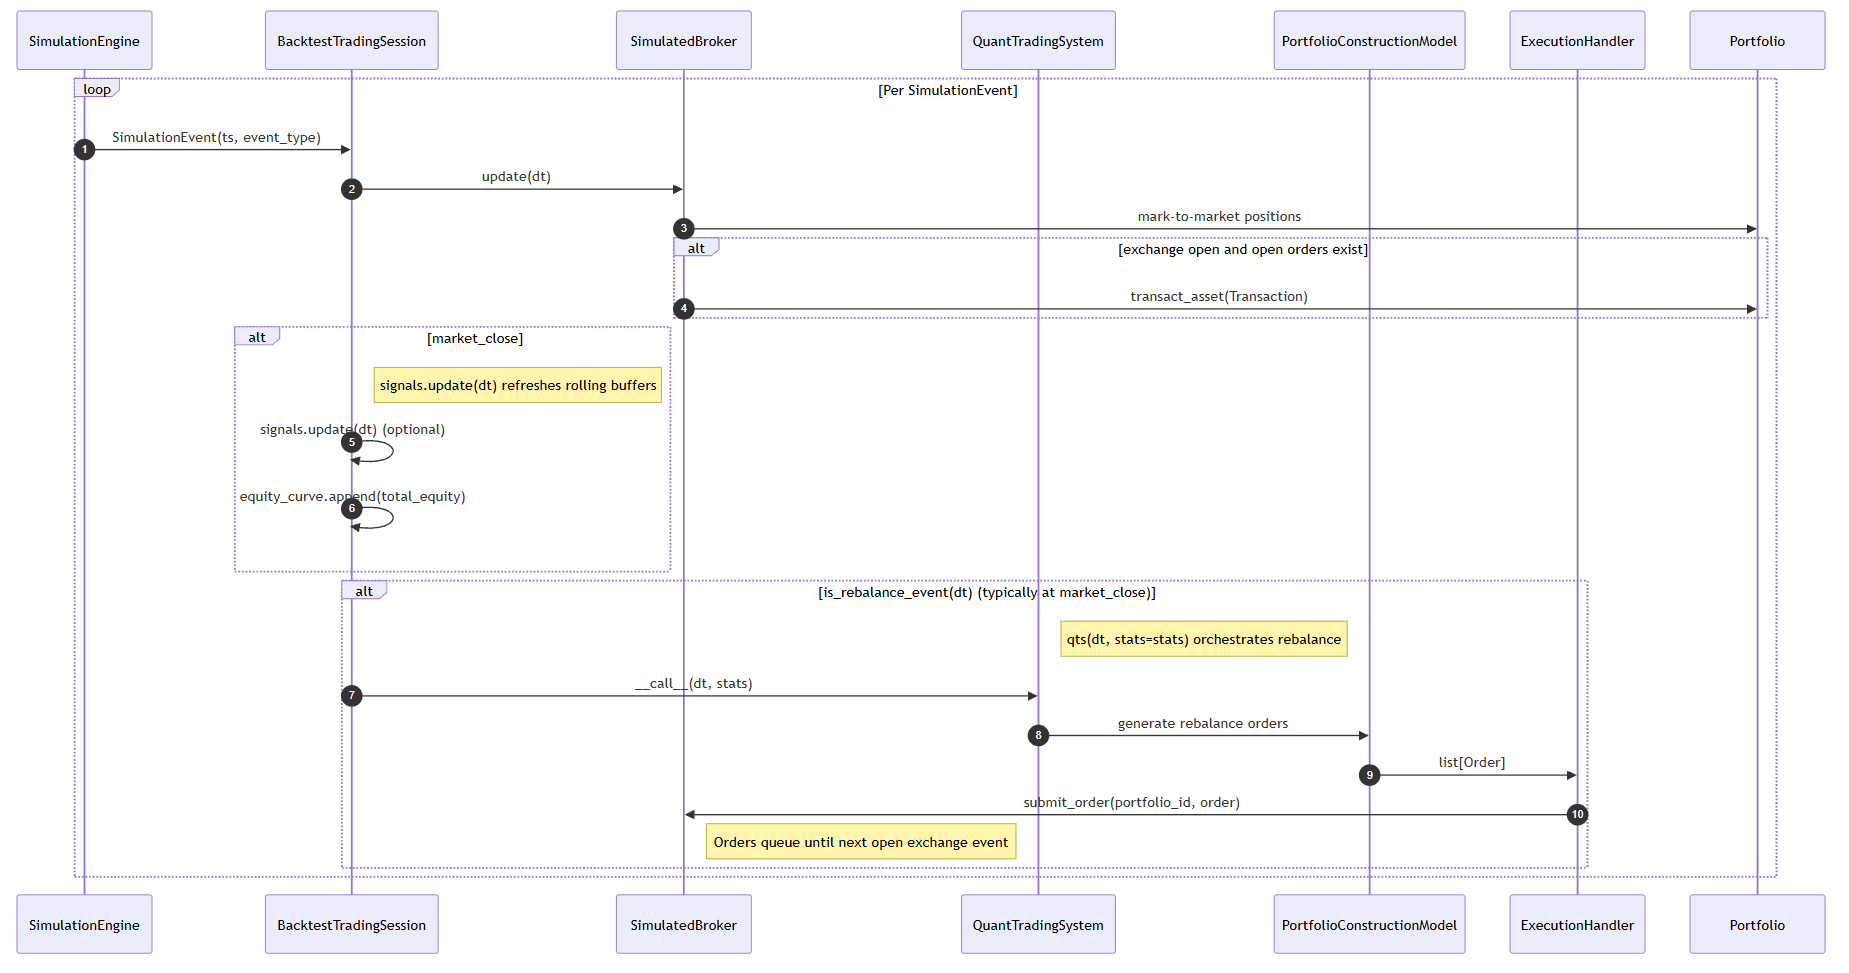
\includegraphics[width=\textwidth,keepaspectratio]{plots/sequence-diagram.png}
\caption{Compact sequence view of the backtest workflow.}
\end{figure}

Timing note:
\begin{itemize}[leftmargin=*]
  \item In the default session, rebalance orders are usually generated/submitted at \texttt{market\_close}, when the exchange is already closed.
  \item Those queued orders are then eligible to fill on the next \texttt{market\_open} \texttt{broker.update(dt)} (subject to exchange-open check).
\end{itemize}

\subsection{Portfolio construction flowchart (tiny)}

\begin{figure}[p]
\centering
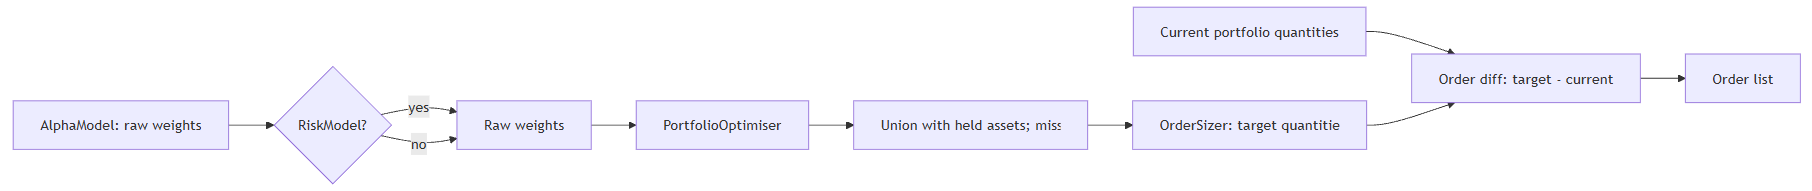
\includegraphics[width=\textwidth,keepaspectratio]{plots/portfolio-construction-flowchart.png}
\caption{Portfolio construction flow from alpha weights to rebalance orders.}
\end{figure}

Legend: \texttt{Current portfolio quantities} is sourced from \texttt{broker.get\_portfolio\_as\_dict(...)}.

\section{Strategy logic (using \texttt{TopNMomentumAlphaModel} as an example)}

\begin{enumerate}[leftmargin=*]
  \item \textbf{Universe} --- All SPDR US sector ETFs (\texttt{XLB}, \texttt{XLC}, \texttt{XLE}, \texttt{XLF}, \texttt{XLI}, \texttt{XLK}, \texttt{XLP}, \texttt{XLU}, \texttt{XLV}, \texttt{XLY}). Because \texttt{XLC} was not listed until June 2018, a \texttt{DynamicUniverse} is used so it is only eligible from that date onwards.
  \item \textbf{Signal} --- 126-business-day (\(\approx\) 6-month) holding-period return momentum, calculated via \texttt{MomentumSignal}.
  \item \textbf{Alpha Model (\texttt{TopNMomentumAlphaModel})} --- At each rebalance event, ranks every eligible asset by its momentum score and assigns an \textbf{equal weight of 1/N} to the top-N assets (\(N = 3\) by default). All other assets receive a weight of 0.
  \item \textbf{Rebalance} --- \texttt{end\_of\_month} (the last trading day of every calendar month).
  \item \textbf{Burn-in} --- The first year of data (1999-01-01) is used purely for signal warm-up; performance statistics begin after that date.
  \item \textbf{Benchmark} --- A static 100\% allocation to SPY using \texttt{FixedSignalsAlphaModel} with a \texttt{buy\_and\_hold} rebalance schedule.
\end{enumerate}

\end{document}

